\documentclass[12pt]{report}
\usepackage[margin=1in]{geometry}
\usepackage{hyperref}
\usepackage{graphicx}
\usepackage{amsmath}
\usepackage{enumitem}
\usepackage{float}

\title{Week 5 Report}
\author{Dhanush Balusa}
\date{June 18, 2025}

\begin{document}

\maketitle

\chapter*{Research}

\textbf{Space-Track.org's Collision Data}
\begin{itemize}
  \item \url{https://www.space-track.org/documents/SFS_Handbook_For_Operators_V1.7.pdf}
  \item Public conjunctions available on Space-Track are generated by the United States Space Command (USSPACECOM), specifically by the 19th Space Defense Squadron (19 SDS).
  \item This is done through daily screenings of the U.S. high-accuracy satellite catalog, which is maintained by the 18th Space Defense Squadron (18 SDS).
  \item When a potential close approach meets or exceeds established risk thresholds, a Conjunction Data Message (CDM) is automatically generated, reviewed, and published to Space-Track.
\end{itemize}

\noindent \textbf{Other resources:}
\begin{itemize}
  \item \url{https://www.space-track.org/documents/CSM_Guide.pdf}
  \item \url{https://www.nasa.gov/cara/frequently-asked-questions/#:~:text=18%20SDS%20operators%20support%20the,posed%20by%20the%20close%20approach.}
  \item From test case \#2: \url{https://ntrs.nasa.gov/api/citations/20070007324/downloads/20070007324.pdf}
\end{itemize}

\chapter*{Code Changes}

Based on the feedback from last week's team meeting, I decided to make the following changes:

\begin{enumerate}
  
  \item \textbf{My first task was to check if other close approaches were modeled accuratley.}
  \newline
  To do this, there was a code change needed to ensure that the TLE is correctly fetched because for some reason the code was erroring with 3 lines of TLE data.
  \newline\newline
  When I first wrote the code, fetching the TLE was erroring because of the 3 lines. This change was made to ensure that the TLE data is correctly formatted and that the \texttt{EarthSatellite} object is created with the correct parameters (by adding the name).
  \newline
  \begin{verbatim}
    tle = [name] + tle_lines
    return EarthSatellite(tle[1], tle[2], tle[0])
  \end{verbatim}

  I had to change the \texttt{fetch\_and\_create\_satellite} function to handle cases where the TLE data might not be available or is incomplete. This ensures that the code does not break when trying to create an \texttt{EarthSatellite} object with insufficient data.
  The code now checks if the TLE lines are less than 2, and if so, it constructs the TLE with the name and the available lines. This prevents errors when trying to create an \texttt{EarthSatellite} object with incomplete data.
  I believe Space-Track.org has changed their API to return TLE data in a different format, which is why the old code errored out.
  \newline
  \begin{verbatim}
    if len(tle_lines) < 2:
        tle = [name] + tle_lines
        return EarthSatellite(tle[0], tle[1])
  \end{verbatim}

  Using the updated code, I was able to successfully fetch the TLEs.

  \pagebreak
  Using Space-Track.org, I was able to find conjunction data for the following test cases from \url{https://www.space-track.org/#/conjunctions}:
  \begin{itemize}
    \item Test Case \#1: COSMOS 2294 \& COSMOS 2288
    \item Test Case \#2: FENGYUN 1C DEBRIS \& NOAA 6
    \item Test Case \#3: COSMOS 468 \& DMSP 5D-2 F13 DEBRIS
    \item Test Case \#4: COSMOS 1816 \& M-4S Rocket Body
  \end{itemize}

  Test case \#1 perfectly matched Space-Track with the Time of Closest Approach (TCA) of 2025-06-20 16:20:00 UTC. This test case is between 2 COSMOS satellites and fetches TLE data 4 days before the alert was created.
  \newline
  URL: \url{https://www.space-track.org/basicspacedata/query/class/cdm_public/cdm_id/1057414232/format/kvn/emptyresult/show}
  \newline
  \begin{figure}[H]
    \centering
    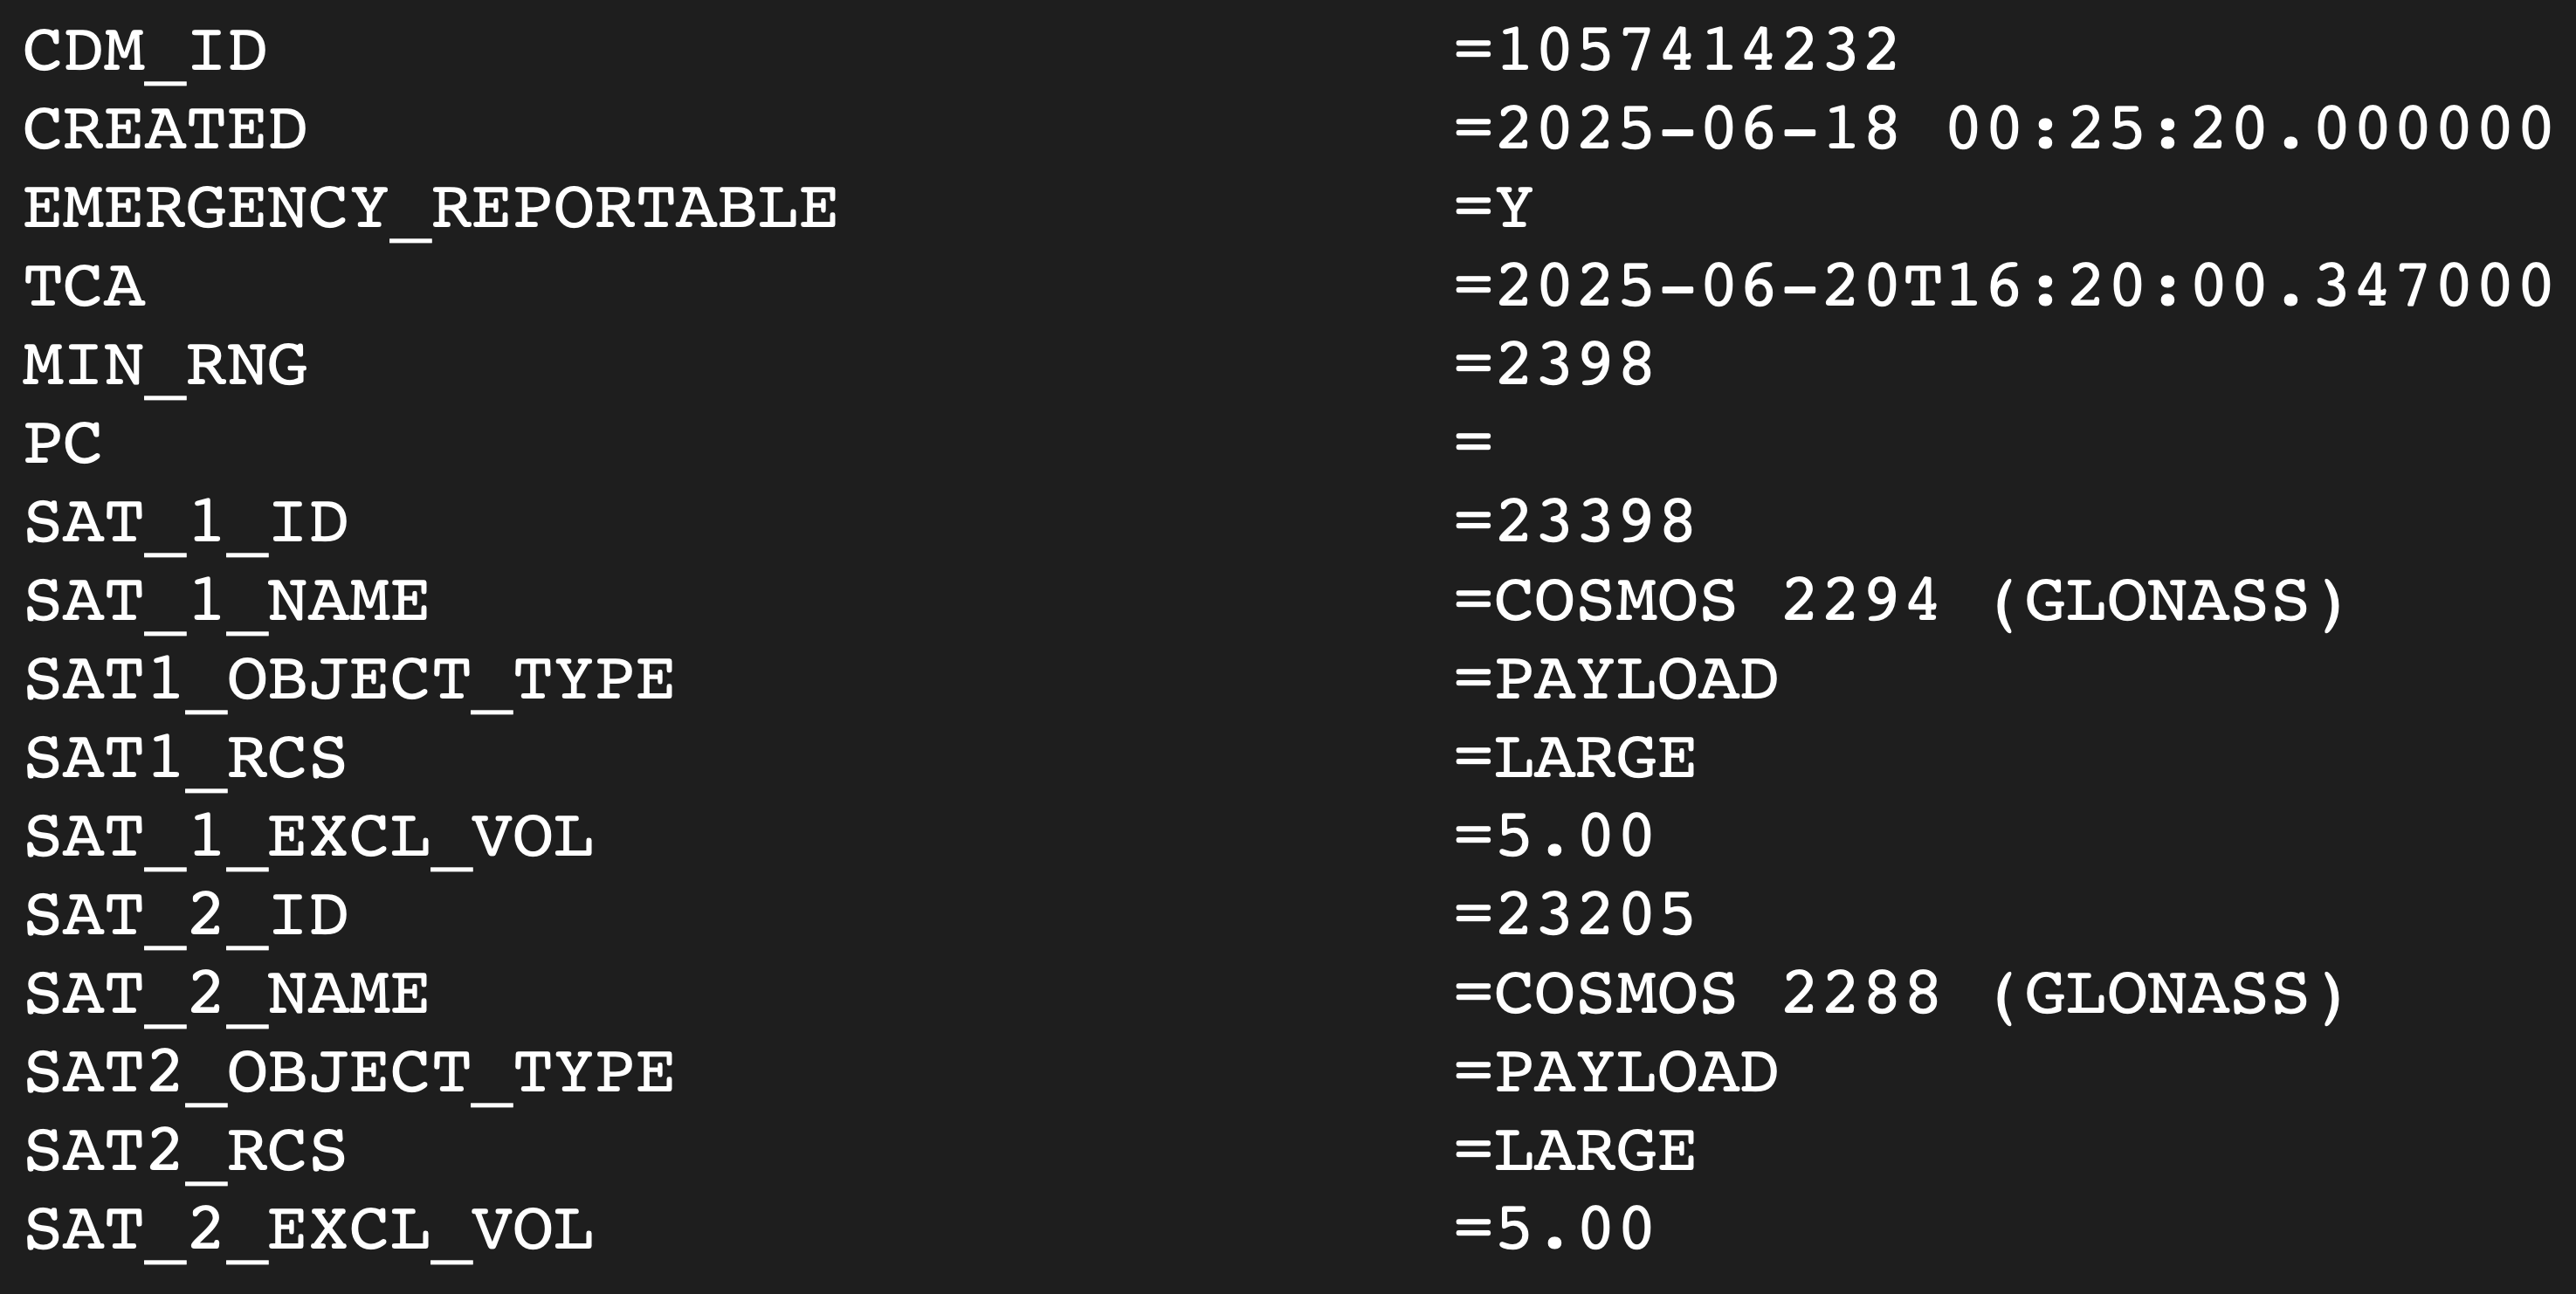
\includegraphics[width=0.8\textwidth]{figure_week_5_test1.png}
    \caption{Test Case \#1: COSMOS 2294 \& COSMOS 2288}
    \label{fig:test_case_1}
  \end{figure}

  \begin{figure}[H]
    \centering
    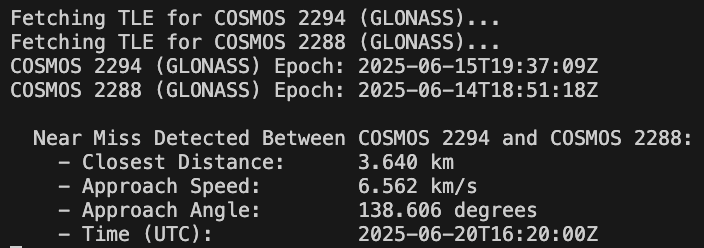
\includegraphics[width=0.8\textwidth]{figure_week_5_test1-output.png}
    \caption{Output of Test Case \#1}
    \label{fig:test_case_1_output}
  \end{figure}

  \begin{figure}[H]
    \centering
    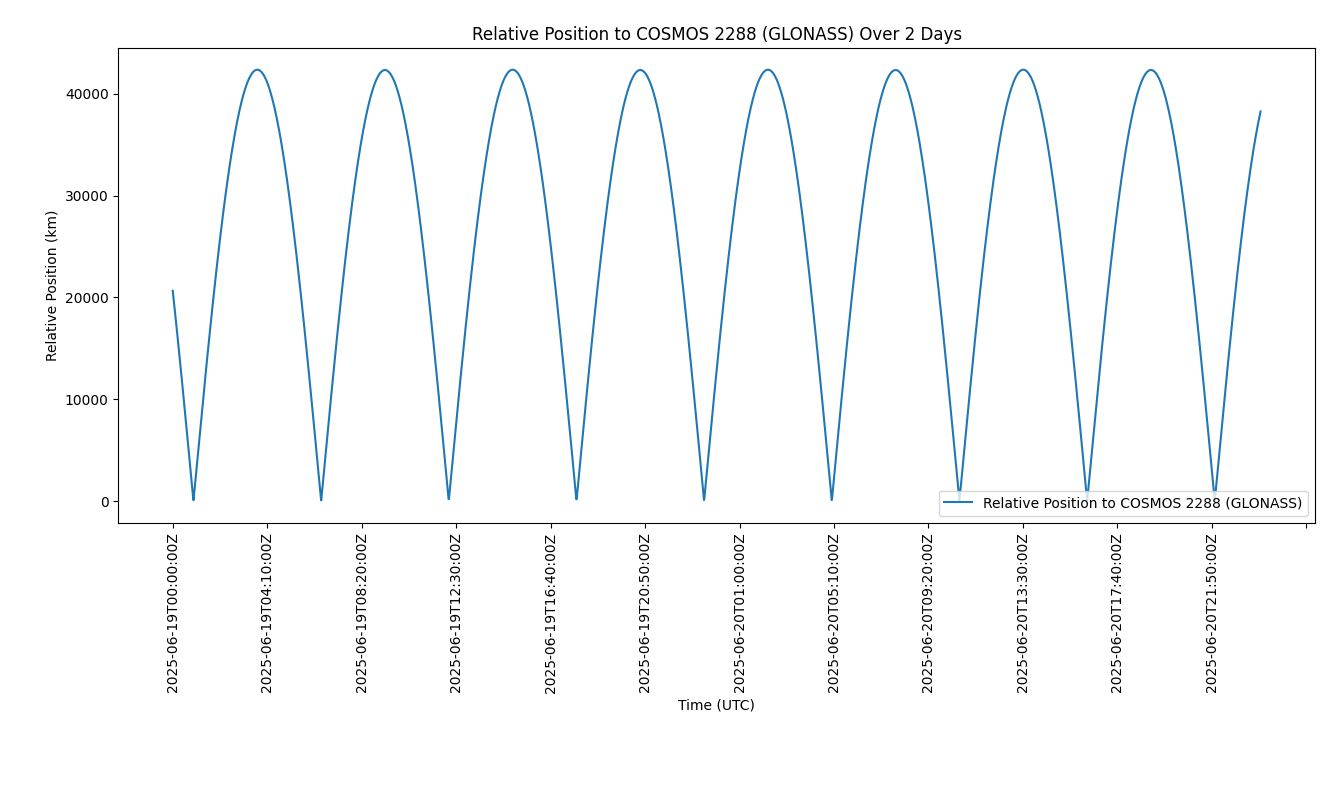
\includegraphics[width=0.8\textwidth]{figure_week_5_test1-graph.png}
    \caption{Graph of Test Case \#1}
    \label{fig:test_case_1_graph}
  \end{figure}

  Test case \#2 perfectly matched Space-Track with the Time of Closest Approach (TCA) of 2025-06-19 19:02:17 UTC. This test case is between a debris from a Chinese anti-missle test and a NOAA satellite and fetches TLE data 1-2 days before the alert was created.
  Initially my calculated TCA was off by 1 hour, but once I increased the time steps, it worked perfectly.
  \newline
  URL: \url{https://www.space-track.org/basicspacedata/query/class/cdm_public/cdm_id/1057084854/format/kvn/emptyresult/show}
  \newline
  \begin{figure}[H]
    \centering
    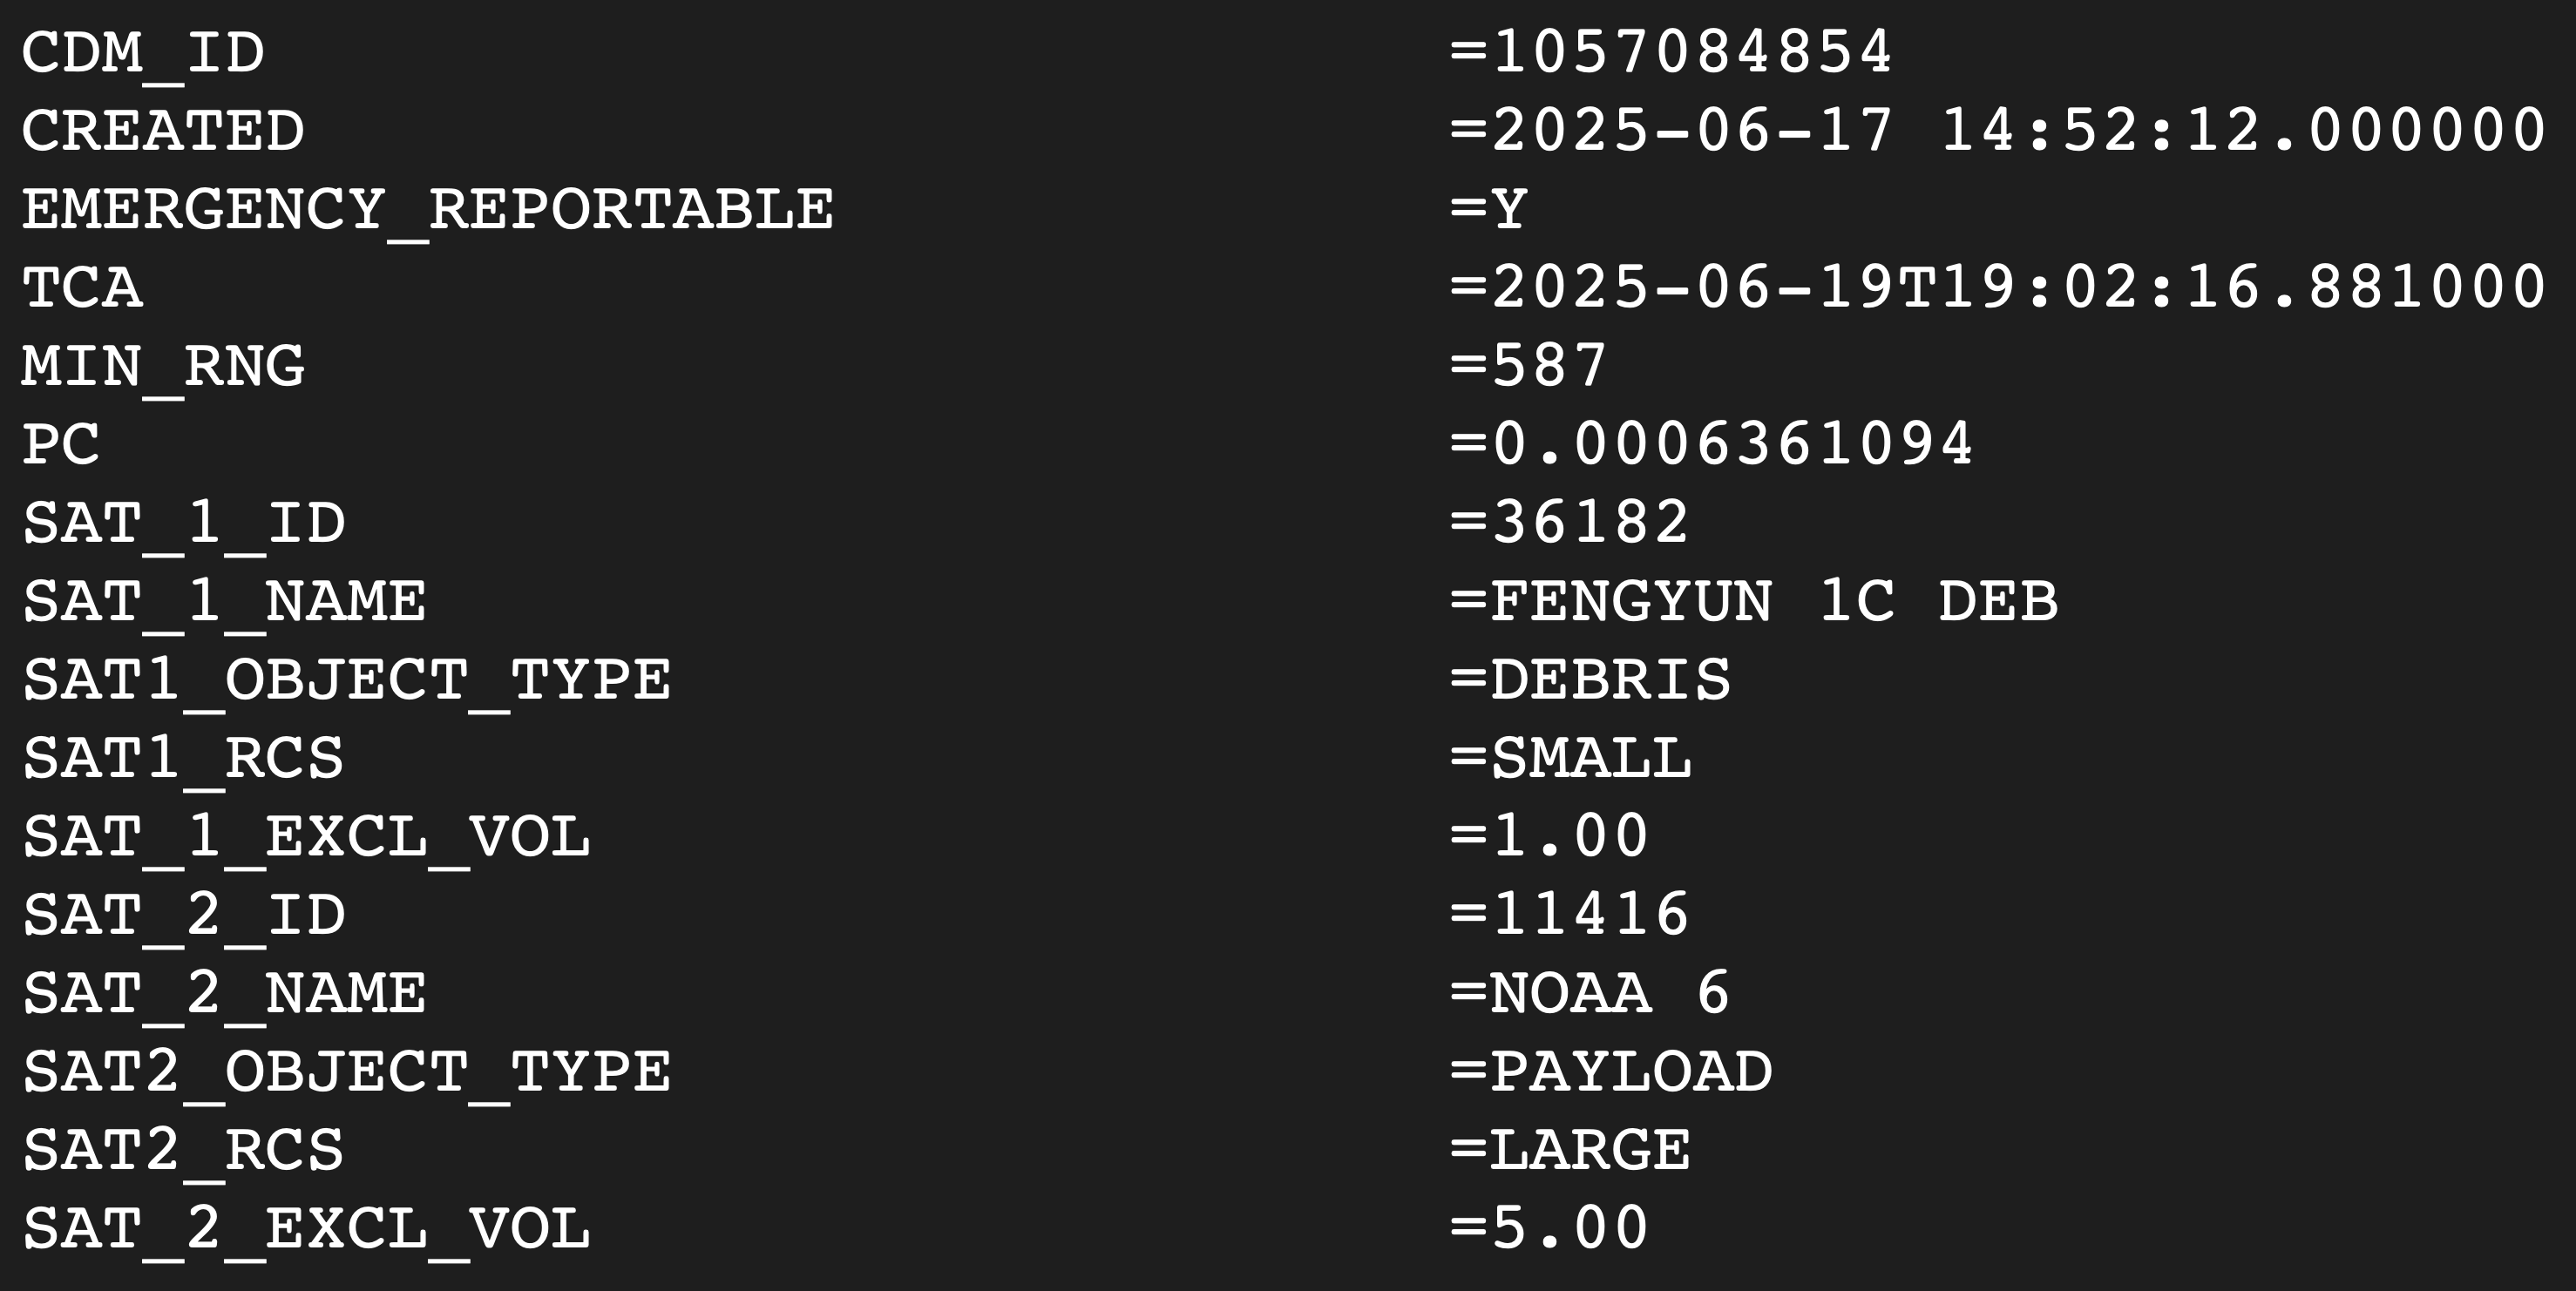
\includegraphics[width=0.8\textwidth]{figure_week_5_test2.png}
    \caption{Test Case \#2: FENGYUN 1C DEBRIS \& NOAA 6}
    \label{fig:test_case_2}
  \end{figure}

  \begin{figure}[H]
    \centering
    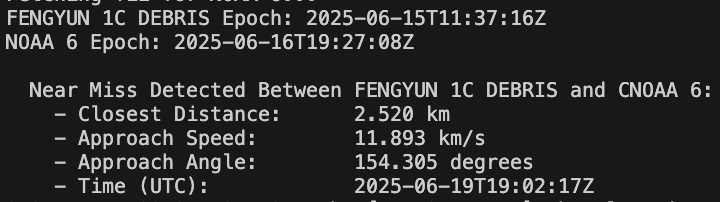
\includegraphics[width=0.8\textwidth]{figure_week_5_test2-output.png}
    \caption{Output of Test Case \#2}
    \label{fig:test_case_2_output}
  \end{figure}

  \begin{figure}[H]
    \centering
    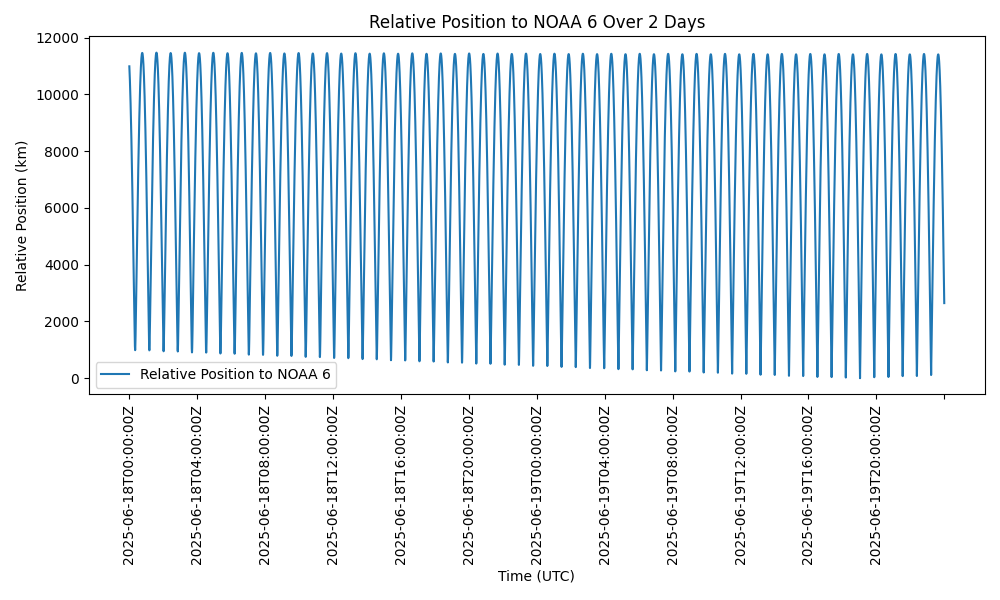
\includegraphics[width=0.8\textwidth]{figure_week_5_test2-graph.png}
    \caption{Graph of Test Case \#2}
    \label{fig:test_case_2_graph}
  \end{figure}

  Test case \#3 wasn't even able to be fetched from Space-Track.org, as it was giving an error that the TLE data was not available for the COSMOS satellite and the debris.
  \newline
  URL: \url{https://www.space-track.org/basicspacedata/query/class/cdm_public/cdm_id/1029160361/format/kvn/emptyresult/show}
  \newline
  \begin{figure}[H]
    \centering
    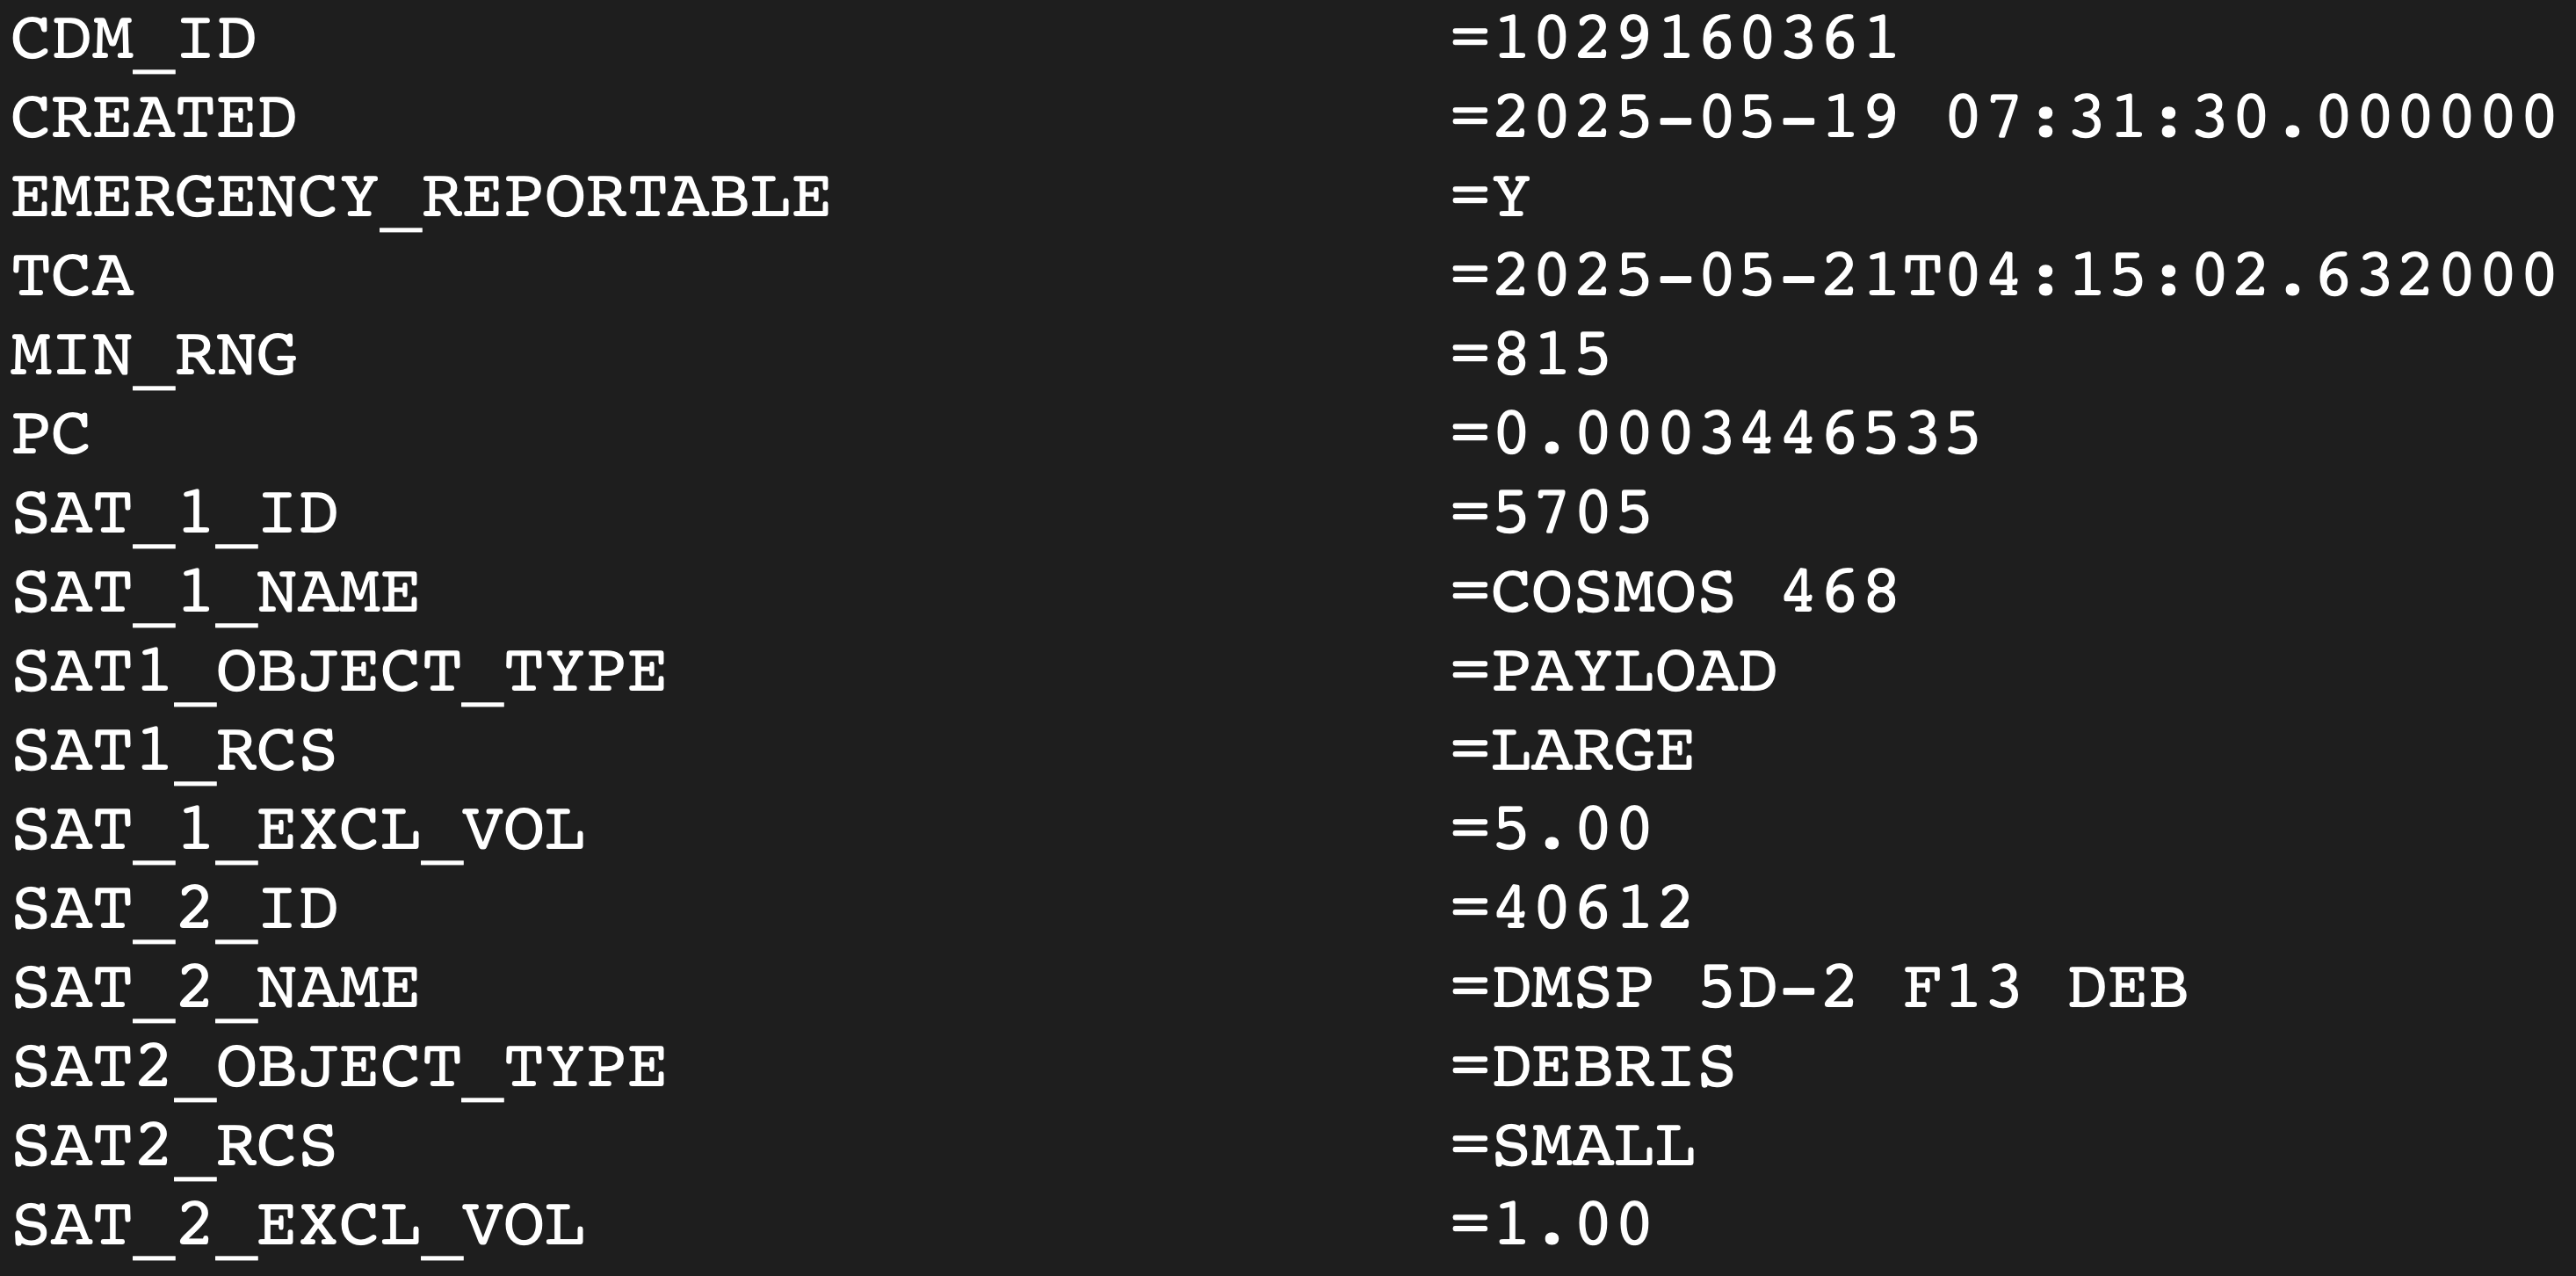
\includegraphics[width=0.8\textwidth]{figure_week_5_test3.png}
    \caption{Test Case \#3: COSMOS 468 - DMSP 5D-2 F13 DEBRIS}
    \label{fig:test_case_3}
  \end{figure}

  \begin{figure}[H]
    \centering
    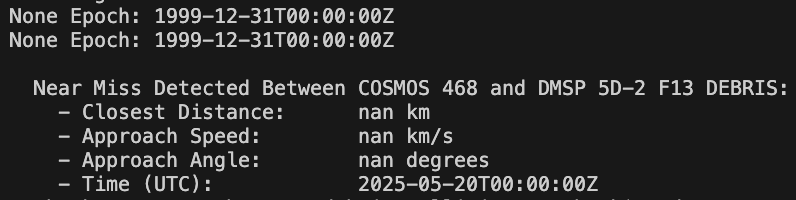
\includegraphics[width=0.8\textwidth]{figure_week_5_test3-output.png}
    \caption{Output of Test Case \#3}
    \label{fig:test_case_3_output}
  \end{figure}

  Test case \#4 also wasn't able to be fetched from Space-Track.org, as it was giving an error that the TLE data was not available for the COSMOS satellite and M-4S Rocket Body.
  \newline
  URL: \url{https://www.space-track.org/basicspacedata/query/class/cdm_public/cdm_id/1056085317/format/kvn/emptyresult/show}
  \newline
  \begin{figure}[H]
    \centering
    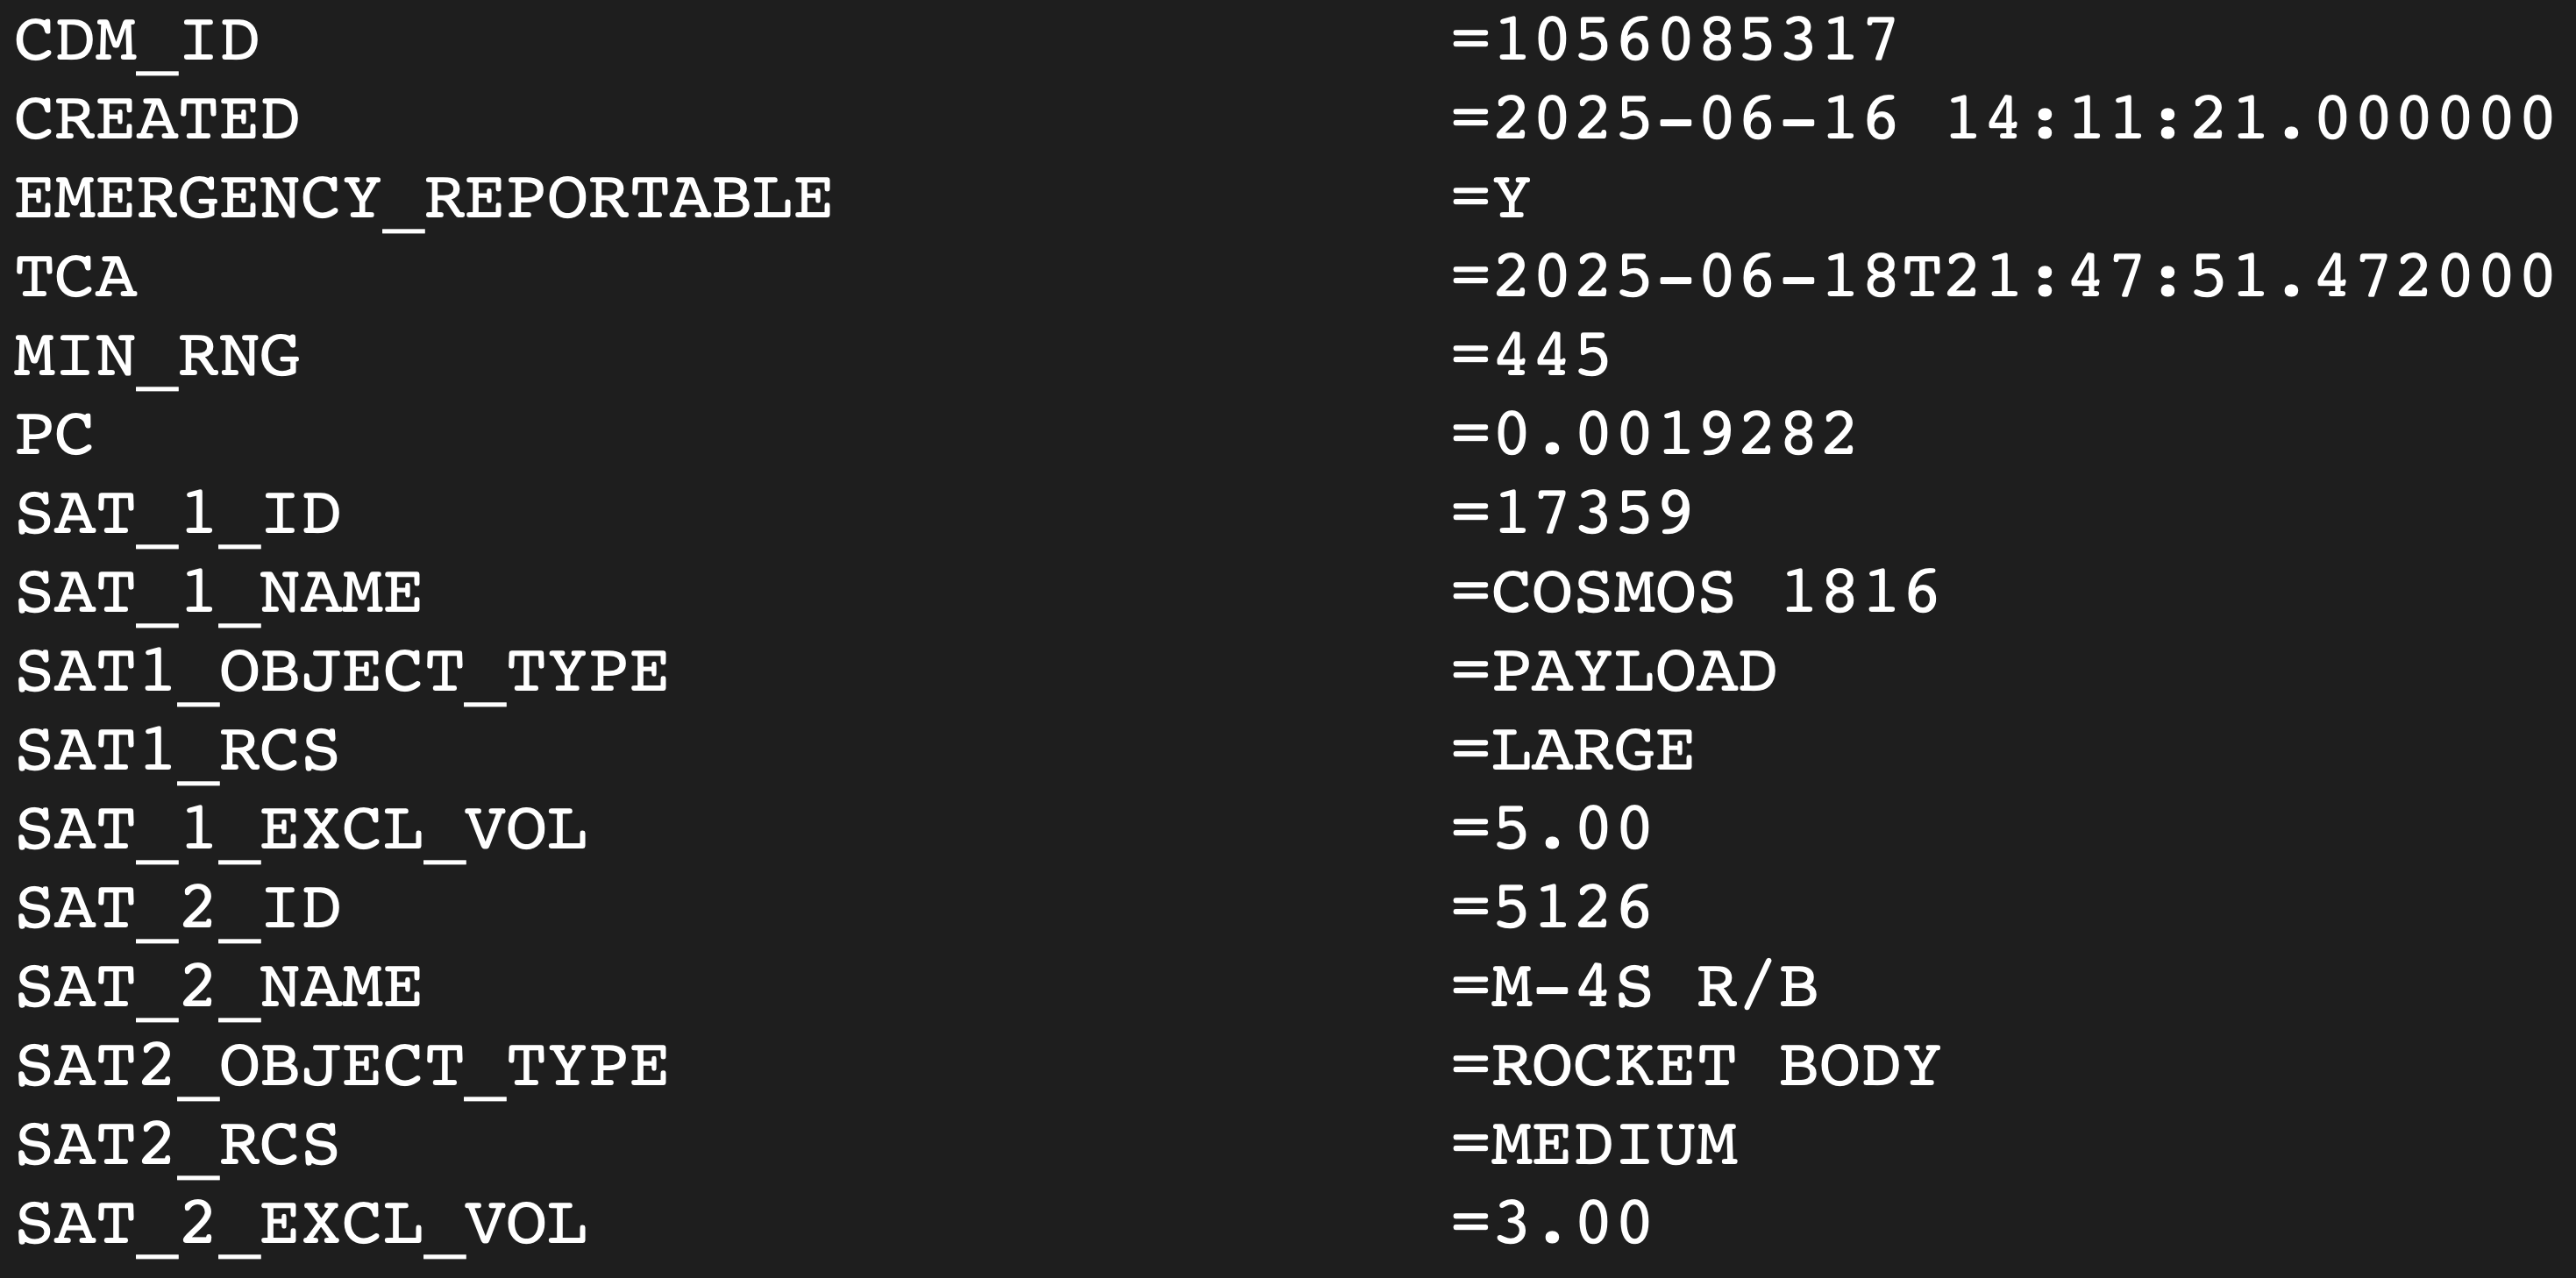
\includegraphics[width=0.8\textwidth]{figure_week_5_test4.png}
    \caption{Test Case \#4: COSMOS 1816 \& M-4S Rocket Body}
    \label{fig:test_case_4}
  \end{figure}

  \begin{figure}[H]
    \centering
    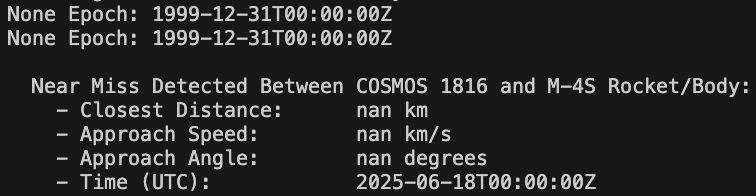
\includegraphics[width=0.8\textwidth]{figure_week_5_test4-output.png}
    \caption{Output of Test Case \#4}
    \label{fig:test_case_4_output}
  \end{figure}

  I went back to the other test cases and found that the TLE data was not available for anything, even from previous weeks' code. This most likely means Space-Track.org has limited my requests to pull TLE data from their API.

  \item \textbf{My second task was to check the approach angle math.}
  \newline\newline
  \textbf{Previous week's approach angle code: }
  \newline
  The code calculates the \textbf{approach angle} between two satellites by measuring the angle between their \textit{relative position vector} and the \textit{velocity vector} with respect to the first satellite (Sat1).
  \newline\newline
  This is computed using the dot product formula:
  \begin{equation}
  \theta = \arccos\left(\frac{\vec{r} \cdot \vec{v}}{|\vec{r}| |\vec{v}|}\right)
  \end{equation}

  where:
  \begin{itemize}
    \item $\vec{r}$ is the relative position vector between the two satellites (from Sat2 to Sat1),
    \item $\vec{v}$ is the relative velocity vector (how fast and in what direction Sat1 is moving relative to Sat2),
    \item $\theta$ is the angle between the two vectors.
  \end{itemize}

  This approach angle provides insight into the geometry of the encounter:
  \begin{itemize}
    \item An angle near $0^\circ$ indicates a \textit{head-on approach}.
    \item An angle near $90^\circ$ suggests a \textit{tangential or glancing pass}.
    \item An angle near $180^\circ$ implies the satellites are moving in \textit{opposite directions}.
  \end{itemize}

  \textbf{Proposed approach angle code: }
  \newline\newline
  The proposed code calculates the \textbf{approach angle} between two satellites by measuring the angle between the \textit{velocity of Sat1} and the \textit{velocity of Sat2}.
  \newline\newline
  This is computed using the dot product formula:
  \begin{equation}
  \theta = \arccos\left(\frac{\vec{v_1} \cdot \vec{v_2}}{|\vec{v_1}| |\vec{v_2}|}\right)
  \end{equation}

  where:
  \begin{itemize}
    \item $\vec{v_1}$ is the velocity vector of Sat1,
    \item $\vec{v_2}$ is the velocity vector of Sat2,
    \item $\theta$ is the angle between the two vectors.
  \end{itemize}

  This approach angle provides insight into the geometry of the encounter:
  \begin{itemize}
    \item An angle near $0^\circ$ indicates a \textit{moving together}.
    \item An angle near $90^\circ$ suggests a \textit{right angle}.
    \item An angle near $180^\circ$ implies the satellites are moving in \textit{head-on collisin}.
  \end{itemize}
  This change was made to ensure that the approach angle is calculated based on the velocities of the satellites, which is more relevant for understanding their relative motion during a close approach.

\end{enumerate}

\chapter*{Next Steps}

\textbf{My notes:}
\begin{itemize}
  \item Look into why test case 3 and 4 are not working.
  \item Test the rest of the cases from Space-Track.org throughout the week to see if I get access again.
  \item Test the proposed approach angle code.
\end{itemize}

\noindent \textbf{Dr. Fan's feedback:}
  \begin{enumerate}
    \item Read approach angle literature. Does not necessarily have to be related to space but can be related to other fields like cars.
    \item Other research on space collision conditions consequence of a collision, break-up model, hypervelocity impact.
    \item Conjunction analysis: 
          \begin{itemize}
            \item How do other people propagate orbit to predict collision?
            \item What other parameters are important in conjunction analysis? Propagation techniques, something else other than TLE data?
          \end{itemize}
  \end{enumerate}

\noindent \textbf{End goals:}
\begin{itemize}
  \item Loop through all the TLEs in the LEO category and calculate the approach conditions for each satellite if it is within a certain distance (e.g., 100 km) of the ISS.
  \item Make my code a usable function so Catherine can just call it. Some input \textrightarrow{} Output (approach speed and angle).
\end{itemize}

\end{document}